\chapter{Progettazione concettuale e logica}
In questo capitolo verranno analizzati i requisiti che deve rispettare il database, e verr\`a quindi definito lo schema Entity-Relationship. Nel caso ci sia la necessit\`a
di definire dei vincoli non esprimibili tramite lo schema ER, verranno inoltre definiti dei vincoli esterni.
\section{Requisiti del database}
L'applicazione prevede la presenza di un Wallet associato a ciascun tenant, che pu\`o essere ricaricato tramite pagamenti effettuati con \textbf{Stripe}.
All'interno del sistema sono previsti dei \textbf{workflow}, processi che utilizzano dati provenienti da banche dati esterne per effettuare analisi di vario tipo.
Ogni operazione all'interno del workflow ha un costo, e per ognuna di queste viene scalato un determinato importo in base a un listino prezzi associato al tenant di appartenenza dell'utente.
Quando un'operazione viene inserita nella coda pagamenti, questa viene processata dal Credit Manager e registrata nel database, e il relativo importo viene scalato automaticamente dal Wallet del tenant.
Deve inoltre essere possibile annullare un'operazione. I listini sono costituiti da una descrizione e una fascia di prezzo, e specificano un importo per ogni tipo di operazione.

\section{Progettazione concettuale}
\subsection{Schema Entity-Relationship}
Uno schema ad alto livello orientato puramente alla definizione dei dati e delle relazioni tra loro, senza fare considerazioni su performance o altro.
Non sono presenti neanche le chiavi primarie normalmente richieste in un vero database.
\begin{figure}[H]
  \centering
  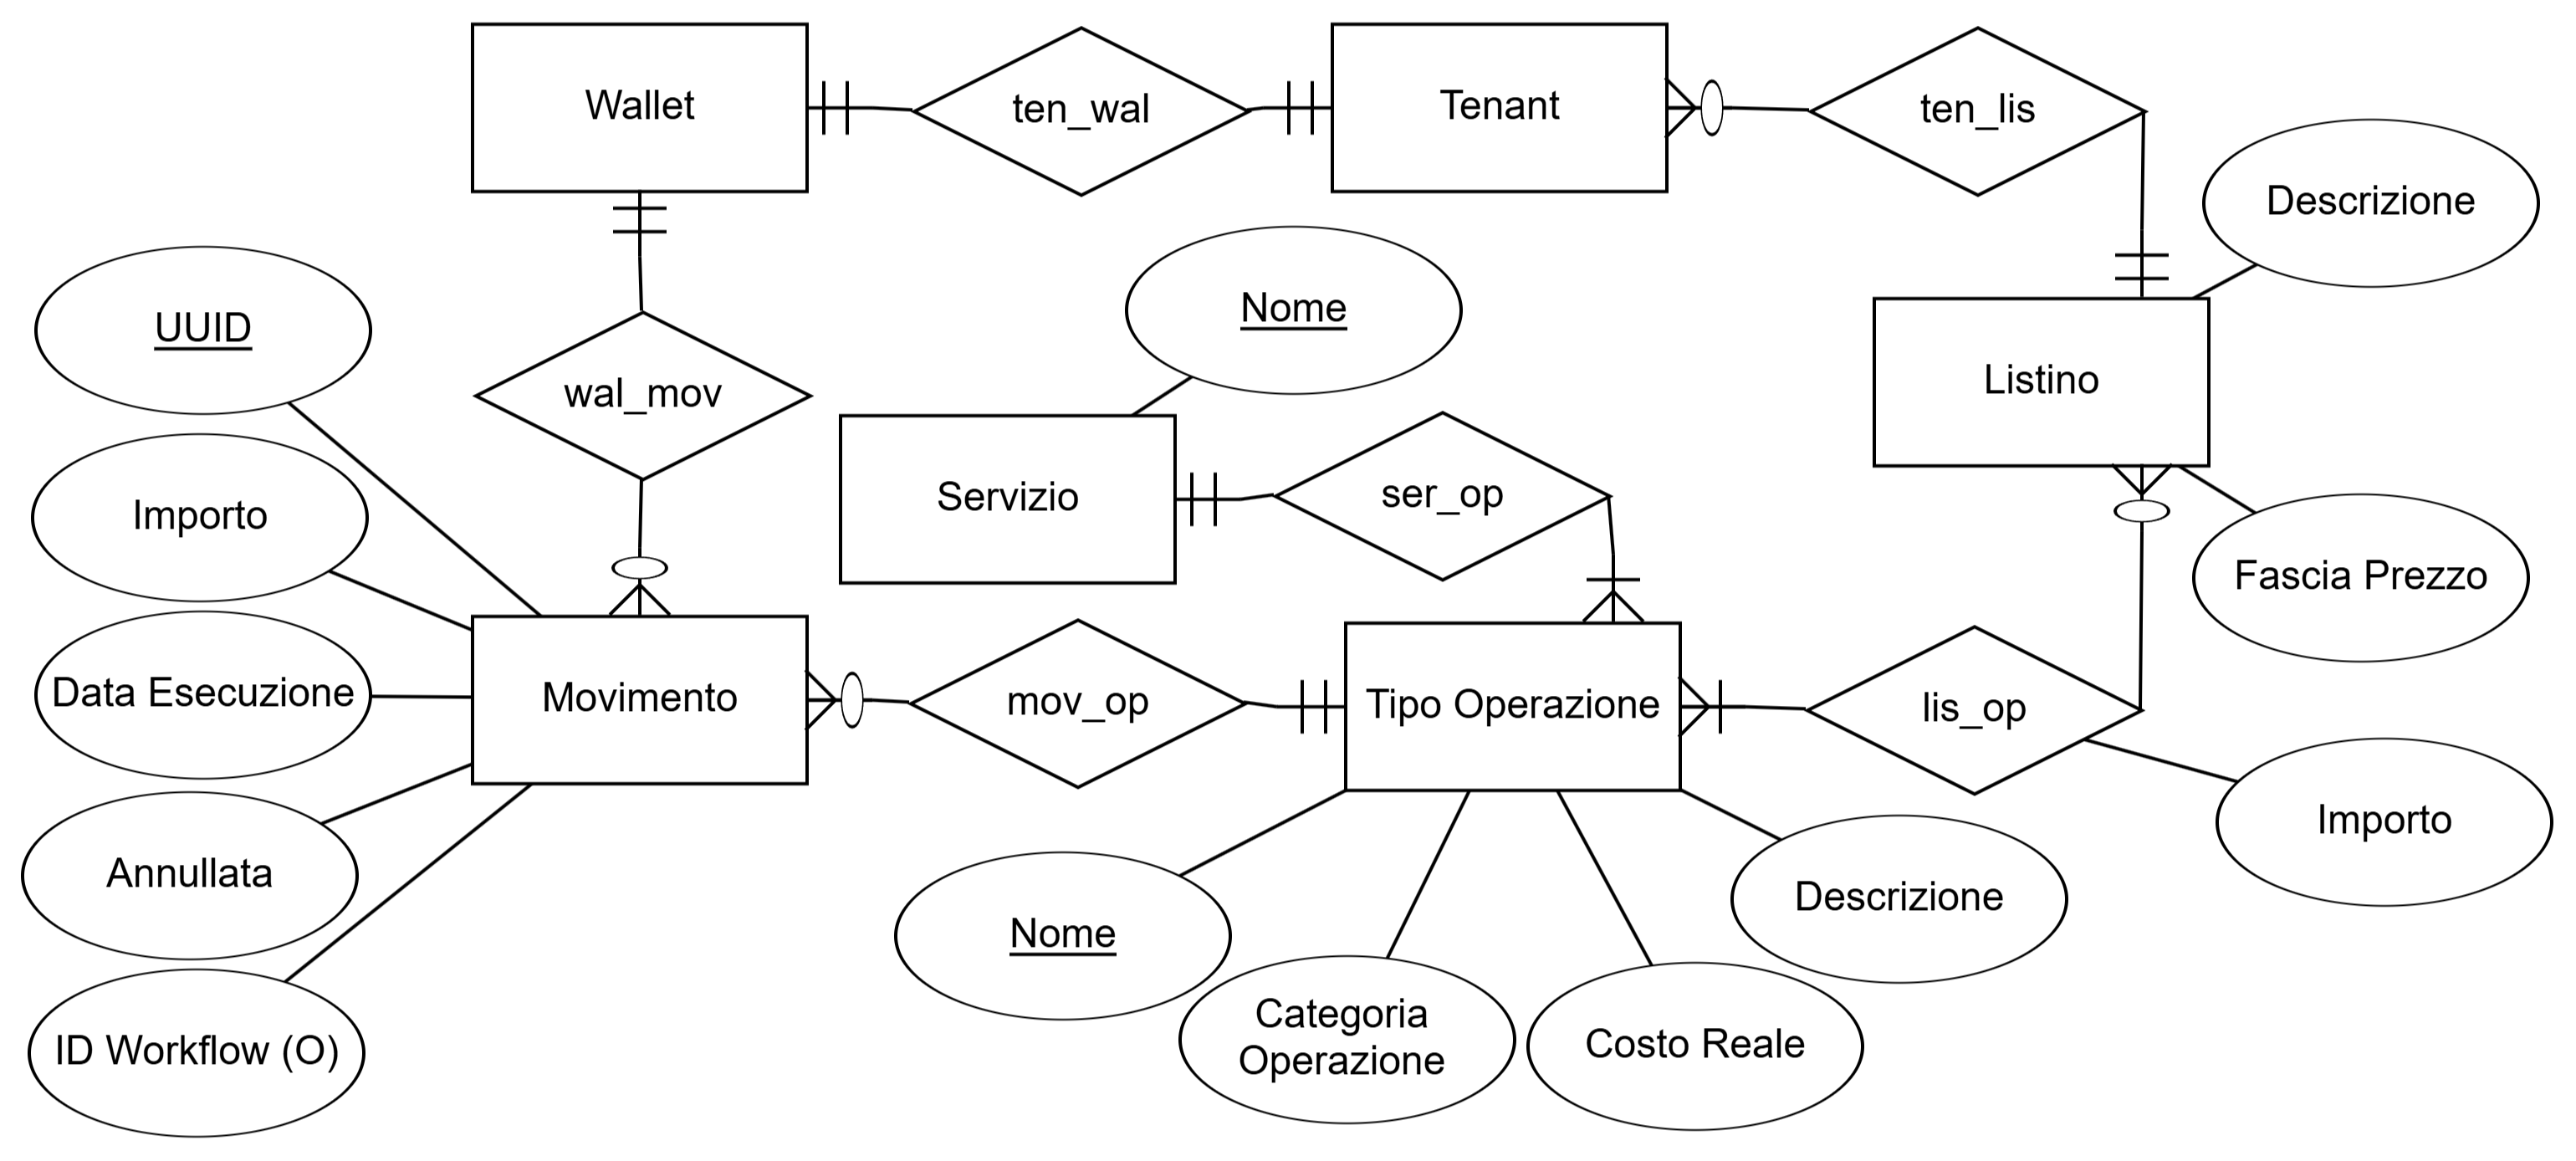
\includegraphics[width=14cm]{images/db-diagrams/er-diagram-concept.png}
  \caption{Schema Entity-Relationship del database}
\end{figure}

\subsubsection{Entit\`a Movimento}
Questa entit\`a rappresenta un singolo movimento. Ogni istanza deve avere una relationship Molti a Uno con Wallet (wal\_mov) e una relationship Molti a Uno con Tipo Operazione (mov\_op).
Pu\`o avere un ID Workflow, se l'operazione \`e stata fatta partire da un Workflow.
\begin{table}[H]
  \centering
  \caption{Descrizione degli attributi dell'entit\`a Movimento}
  \begin{tabulary}{0.9\textwidth}{p{3cm}p{2cm}L}
    \toprule
    \textbf{Attributo} & \textbf{Dominio} & \textbf{Descrizione} \\
    \midrule
    UUID & UUID & UUID dell'operazione all'interno del workflow \\\addlinespace
    Importo & Numeric & Importo pagato dall'utente \\\addlinespace
    Data Esecuzione & DataOra & Data e Ora di esecuzione del movimento \\\addlinespace
    ID Workflow & integer & Identificatore del Workflow di cui fa parte il movimento \\\addlinespace
    Annullata & booleana & Indica che l'operazione \`e stata annullata e ha un'operazione contraria che la bilancia \\\bottomrule
  \end{tabulary}
\end{table}

\subsubsection{Entit\`a Servizio}
Rappresenta uno dei servizi che Sentinel pu\`o interrogare, o Sentinel stesso. Ha una relationship Uno a Molti con Tipo Operazione (ser\_op).
\begin{table}[H]
  \centering
  \caption{Descrizione degli attributi dell'entit\`a Servizio}
  \begin{tabulary}{\textwidth}{LLL}
    \toprule
    \textbf{Attributo} & \textbf{Dominio} & \textbf{Descrizione} \\
    \midrule
    Nome & Stringa & Nome del Servizio \\\bottomrule
  \end{tabulary}
\end{table}

\subsubsection{Entit\`a Tipo Operazione}
Entit\`a che rappresenta il Tipo Operazione, cio\`e le operazioni eseguibili che comportano un addebito o un accredito. Ha una relationship Molti a Uno con Servizio (ser\_op)
che rappresenta il Servizio su cui viene svolta l'operazione, o Sentinel stesso per ricariche o annullamenti. Inoltre ha una relationship Molti a Molti con Listino (lis\_op).
\begin{table}[H]
  \centering
  \caption{Descrizione degli attributi dell'entit\`a Tipo Operazione}
  \begin{tabulary}{0.9\textwidth}{p{2.3cm}p{2.7cm}L}
    \toprule
    \textbf{Attributo} & \textbf{Dominio} & \textbf{Descrizione} \\
    \midrule
    Nome & Stringa & Nome del Tipo Operazione \\\addlinespace
    Categoria Operazione & \{ADDEBITO, ACCREDITO\} & Tipologia di operazione. Utilizziamo un enum type per rappresentare questo attributo. \\\addlinespace
    Costo Reale & numeric & Costo reale affrontato interrogando la banca dati esterna \\\addlinespace
    Descrizione & Stringa & Breve descrizione di cosa fa l'operazione\\\bottomrule
  \end{tabulary}
\end{table}

\subsubsection{Entit\`a Listino}
In questa entit\`a vengono rappresentati i Listini creati dall'amministratore. Un Listino pu\`o avere una relationship Uno a Molti con Tenant (ten\_lis), e deve avere delle
relationship Molti a Molti (lis\_op) con Tipo Operazione.

\begin{table}[H]
  \centering
  \caption{Descrizione degli attributi dell'entit\`a Listino}
  \begin{tabulary}{\textwidth}{p{2.3cm}p{1.8cm}L}
    \toprule
    \textbf{Attributo} & \textbf{Dominio} & \textbf{Descrizione} \\
    \midrule
    Descrizione & Stringa & Descrizione del Listino\\
    Fascia Prezzo & \{ALTA, MEDIA, BASSA\} & Campo descrittivo per indicare la fascia di prezzo del listino\\\bottomrule
  \end{tabulary}
\end{table}

\subsubsection{Relationship lis\_op}
Relationship che rappresenta l'importo che deve venire scalato dal Wallet di un Tenant quando viene registrato un movimento.
Uno dei requisiti \`e che ogni Listino deve specificare un importo per ogni Tipo Operazione. Non essendo possibile forzare la presenza di una relationship tra ogni
istanza di Listino e ogni istanza di Tipo Operazione attraverso lo schema ER, verr\`a disposto un vincolo esterno.

\begin{table}[H]
  \centering
  \caption{Descrizione degli attributi della relationship lis\_op}
  \begin{tabulary}{\textwidth}{p{2.3cm}p{2.3cm}L}
    \toprule
    \textbf{Attributo} & \textbf{Dominio} & \textbf{Descrizione} \\
    \midrule
    Importo & numeric & Importo che verr\`a scalato al tenant associato al listino prezzi\\\bottomrule
  \end{tabulary}
\end{table}

\subsection{Vincoli Esterni}
Dalla costruzione dello schema concettuale \`e emersa la necessit\`a di rappresentare il seguente vincolo esterno:
\subsubsection{\label{tuttiimporticoncept}Tutti gli importi specificati}
$ \forall l, \forall t (Listino(l) \land TipoOperazione(t) \implies lis\_op(l, t)) $\\
Esiste una relationship lis\_op tra ogni entit\`a Listino e ogni entit\`a Tipo Operazione.

\section{Casi d'uso}
In questa sezione verr\`a fornito lo schema UML dei casi d'uso, che indica le funzionalit\`a dell'applicazione e gli attori che le useranno. Prenderemo inoltre in esame
un caso d'uso rappresentativo all'interno dell'applicativo e rappresenteremo le sue specifiche.
\begin{figure}[H]
  \centering
  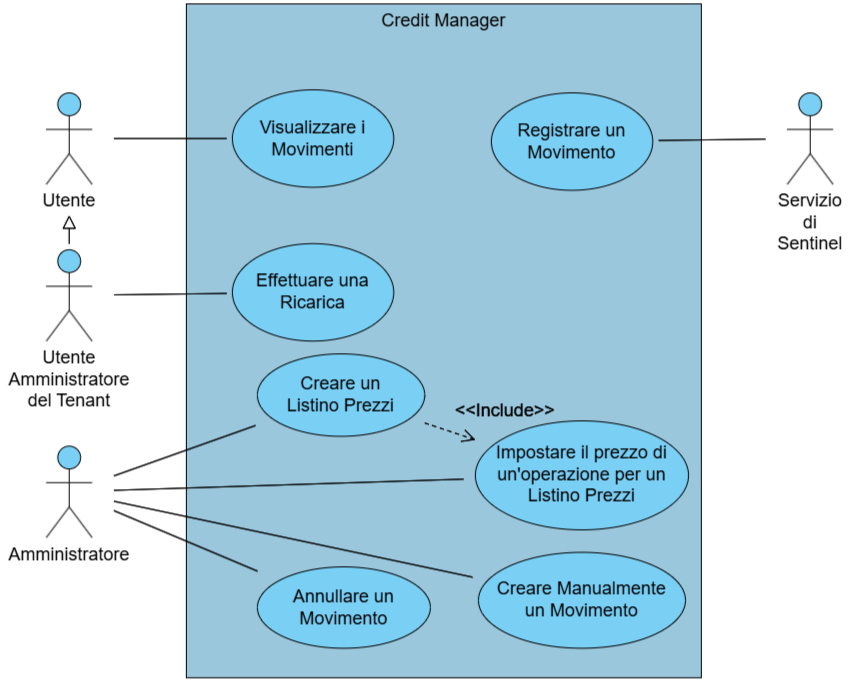
\includegraphics[width=13cm]{images/db-diagrams/use-case-diagram.jpg}
  \caption{Schema UML dei casi d'uso}
\end{figure}
\newpage
\subsubsection{Specifica dei casi d'uso di Crea Listino}
Specifichiamo come dovr\`a funzionare l'operazione per creare un listino prezzi:

\textbf{crea\_listino(descrizione: Stringa, fascia\_prezzo: \{ALTA, MEDIA,\\BASSA\}, tipi\_operazione: [TipoOperazione], prezzi: [Numeric]) $\implies$ Listino:}

\textit{pre}:\\
\hspace*{0.5 cm}Verifica le seguenti condizioni:
\begin{itemize}
  \item $descrizione \neq$ ``''
  \item $tipi\_operazione.length == prezzi.length$
  \item $\forall tipoOperazione \in Tipo Operazione \implies \exists op \in tipi\_operazione \land op == tipoOperazione $
\end{itemize}
\textit{post}:
\begin{enumerate}
  \item Crea un nuovo Listino con la descrizione e fascia prezzo.
  \item Per ogni \textit{tipo} in \textit{tipo\_operazione} crea una nuova relationship PrezzoListino tra il nuovo listino e \textit{tipo},
    con importo uguale all'elemento di \textit{prezzi} con lo stesso indice.
  \item Restituisci il nuovo Listino
\end{enumerate}

Verr\`a fornita un'implementazione nella \textbf{Sezione \ref{crealistinosection}}.
